% @Author: Taha Bouhsine


%%%%%%%%%%%%%%%%%%%%%%%%%%%%
% CHAPTER                  %
%%%%%%%%%%%%%%%%%%%%%%%%%%%%
\setcounter{mtc}{11}

\chapter{Realization, GUI And Tests}%
\label{chap:chapter_four}
\minitoc

\section{Hardware Environments}

\begin{figure}[!ht]
      \centering
      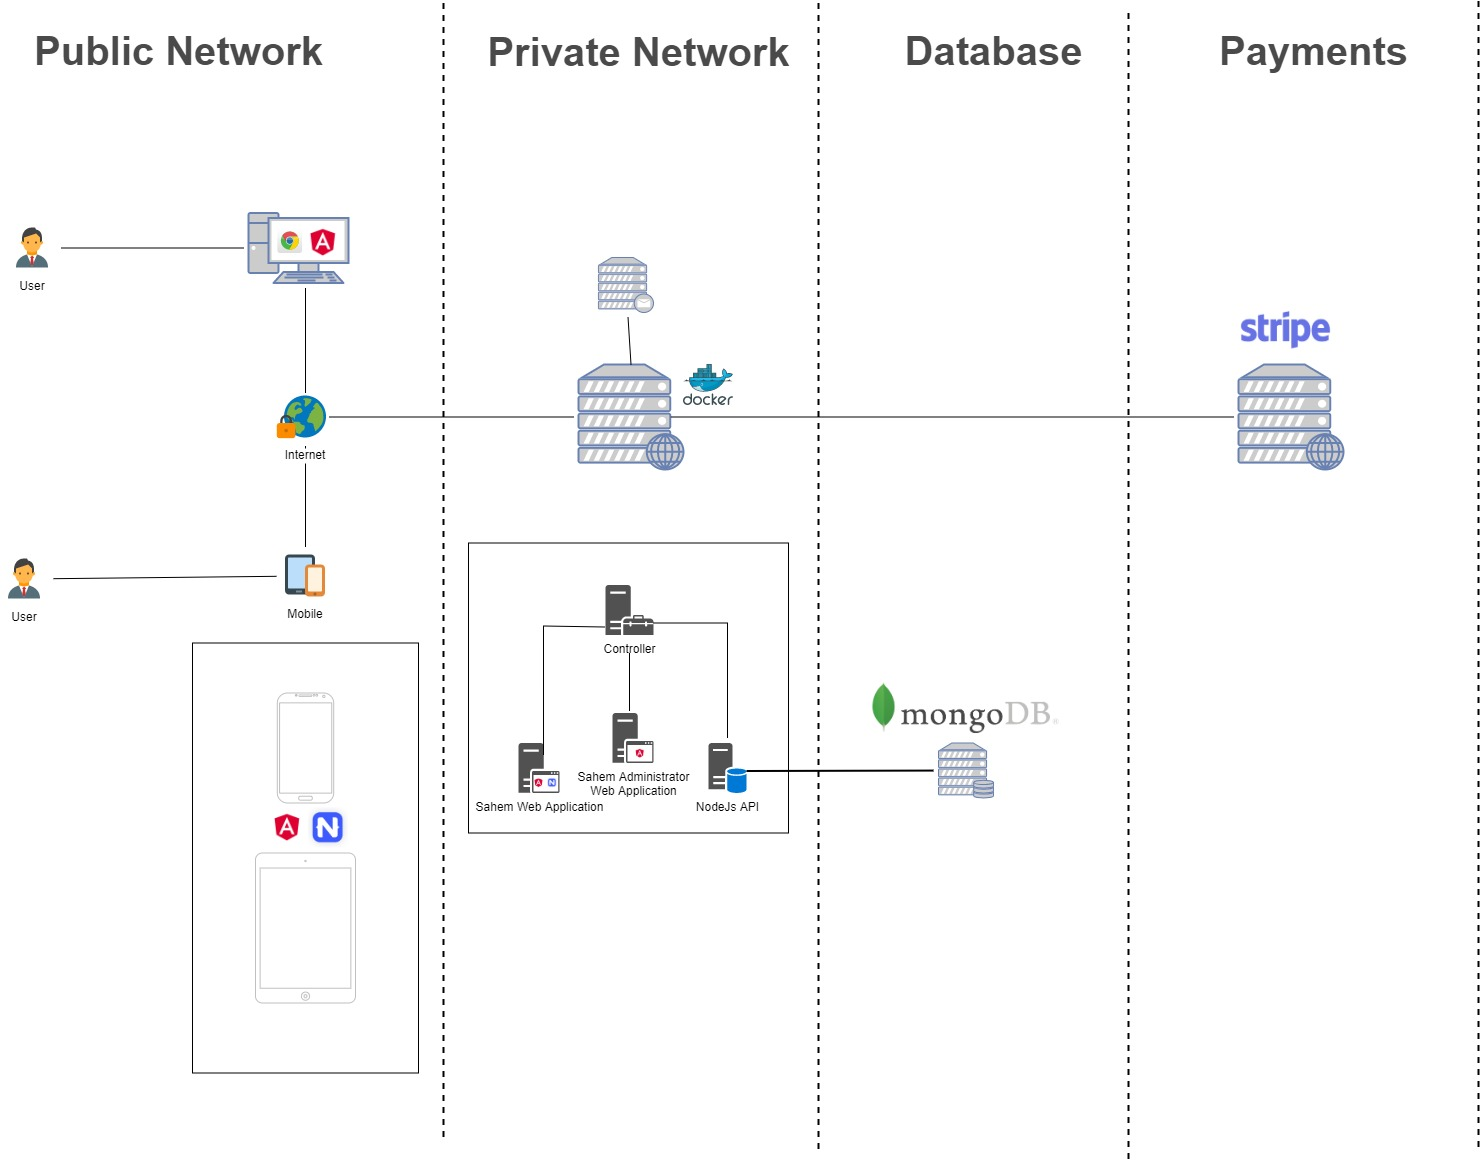
\includegraphics[scale=0.30]{assets/architecturedrawio.jpg}
      \caption{Sahem Platform's Hardware Architecture}
      \label{fig:sahemarchitecturedrawio}
\end{figure}

\section{Development Environments}
\subsection{Design And Planing}

\paragraph*{PlantUml}
In the modeling phase, we found many other solutions and softwares that helped to create diagrams, but they all are graphic based solutions, you have to drag and drop lot of objects, draging arrows from one class to the other, which we found it to be frustrating and tiring with time, so we have decided to go with Plant Uml. We are programers and we should use that fact.\\
PlantUML is an open-source tool allowing users to create UML diagrams from plain text language. The language of PlantUML is an example of a Domain-specific language. It uses Graphviz software to lay out its diagrams. It has been used to allow blind students to work with UML. PlantUML also helps blind software engineers to design and read UML diagrams.


\paragraph*{Gantt chart}
A Gantt chart is a horizontal bar chart that visually represents a project plan over time. Modern Gantt charts typically show us the status of—as well as who’s responsible for—each task in the project.\\

In other words, a Gantt chart is a super-simple way to keep us out of a project pinch!\\

A Gantt chart is made up of several different elements:
\begin{enumerate}
      \item
            Tasklist: Runs vertically down the left of the Gantt chart to describe project work and may be organized into groups and subgroups
      \item
            Timeline: Runs horizontally across the top of the Gantt chart and shows months, weeks, days, and years
      \item
            Dateline: A vertical line that highlights the current date on the Gantt chart
      \item
            Bars: Horizontal markers on the right side of the Gantt chart that represent tasks and show progress, duration, and start and end dates
      \item
            Milestones: Yellow diamonds that call out major events, dates, decisions, and deliverables
      \item
            Dependencies: Light gray lines that connect tasks that need to happen in a certain order
      \item
            Progress: Shows how far along work is and may be indicated by \% Complete and/or bar shading
      \item
            Resource assigned: Indicates the person or team responsible for completing a task
\end{enumerate}


\subsection{User Interface And Product Design}
\paragraph*{Adobe Photoshop}
Adobe Photoshop is a software application for image editing and photo retouching for use on Windows or macOS computers. Photoshop offers users the ability to create, enhance, or otherwise edit images, artwork, and illustrations. Changing backgrounds, simulating a real-life painting, or creating an alternative view of the universe are all possible with Adobe Photoshop. It is the most widely used software tool for photo editing, image manipulation, and retouching for numerous image and video file formats. The tools within Photoshop make it possible to edit both individual images as well as large batches of photos.
We used it to prototype and create our platform logo.
\paragraph*{Adobe XD}
Adobe XD is a vector-based user experience design tool for web apps and mobile apps, developed and published by Adobe Inc. It is available for macOS and Windows, although there are versions for iOS and Android to help preview the result of work directly on mobile devices. XD.






\subsection{Development}
\subsubsection{Version Control}
When building software it’s always important to track your changes. This is especially critical when collaborating on projects where multiple people will be updating the same code. Software that can keep track of all
these changes is called Version Control. The Version Control software we used is called Git. Because we built
the platform for a client we decided to get a private repository at Github.com.

\paragraph*{Git}
% Git is a version control system for tracking changes in computer files and coordinating work on those files among multiple people. It is primarily used for source code management in software development, but it can be used to keep track of changes in any set of files. As a distributed revision control system it is aimed at speed, data integrity, and support for distributed, non-linear workflows.
Git is a distributed revision control and source code management system that
allows several people to work on the same codebase at the same time on different
computers and networks. These can be pushed together, with all changes stored and
recorded. It’s also possible to roll back to an earlier state if necessary.
\paragraph*{Github}
At a high level, GitHub is a website and cloud-based service that helps developers store and manage their code, as well as track and control changes to their code. To understand exactly what GitHub is, we need to know two connected principles:
\begin{enumerate}
      \item Version control
      \item Git
\end{enumerate}

\paragraph{Github Desktop}
GitHub Desktop is a fast and easy way to contribute to projects from Windows and OS X, whether we are seasoned users or new users, GitHub Desktop is designed to simplify all processes and workflow in our GitHub. GitHub Desktop is an open-source Electron-based GitHub app. It is written in TypeScript and uses React.


\subsubsection{Dependency Managers}
A large software project often makes use of many third-party packages and libraries. In turn, these packages
often rely on several other packages and so on. To keep track of all these dependencies, software developers
use package managers. Below we introduce the ones we have used.
\paragraph*{NPM}
\paragraph*{Angular CLI}

\subsubsection{IDEs}

\paragraph*{Visual Studio Code}
Visual Studio Code is a source code editor developed by Microsoft for Windows, Linux and macOS. It includes support for debugging, embedded Git control and GitHub, syntax highlighting, intelligent code completion, snippets, and code refactoring.


\paragraph*{MongoDB Compass Community}
MongoDB Compass is the defacto GUI tool for MongoDB much like MySQL Workbench is MySQL’s associated tool. It allows us to visually explore our data, run ad hoc queries, interact with our data with full CRUD functionality, as well as view and optimize our queries’ performance.


\paragraph*{Postman}
Postman is an interactive and automatic tool for verifying the APIs of our project. Postman is a Google Chrome app for interacting with HTTP APIs. It presents us with a friendly GUI for constructing requests and reading responses. It works on the backend, and makes sure that each API is working as intended.

In Postman, we create a request, and Postman looks at the response to make sure it has the element we want in it. As it is an automation tool, it drastically improves the testing time and quality of the project. It helps in the early detection of bugs that might sprout at later stages and cause more damage to the system.

Postman is the way to streamline the process of API testing. All APIs that we create and deploy first rigorously go through Postman so that any major or show stopper bugs are identified on time and fewer bugs leak through to later stages.




\subsubsection{Report And Presentation}
\paragraph*{Boost Note}
Boostnote is an Open source note-taking app for programmers.
Boostnote is a niche tool because designed for programmers, but we are passionate for it.
It focuses on writing Markdown notes and code snippets quickly, and get organized in a better way.

\paragraph*{Latex}
\latex{} is a tool used to create professional-looking documents. It is based on the WYSIWYM (what we see is what we mean) idea, meaning we only have to focus on the contents of our document and the computer will take care of the formatting. Instead of spacing out text on a page to control formatting, as with Microsoft Word or LibreOffice Writer, users can enter plain text and let LATEX take care of the rest.
\paragraph*{MiKTex}
MiKTeX provides the tools necessary to prepare documents using the TeX/LaTeX markup language, as well as a simple tex editor: TeXworks.

\paragraph*{Tex Live}
TeX Live is intended to be a straightforward way to get up and running with the TeX document production system. It provides a comprehensive TeX system with binaries for most flavors of Unix, including GNU/Linux, macOS, and also Windows. It includes all the major TeX-related programs, macro packages, and fonts that are free software, including support for many languages around the world. Many operating systems provide it via their distributions.



\paragraph*{Markdown}
Markdown is a lightweight markup language with plain-text-formatting syntax. Its design allows it to be converted to many output formats, but the original tool by the same name only supports HTML. Markdown is often used to format readme files, for writing messages in online discussion forums, and to create rich text using a plain text editor.
\paragraph*{Marp}
Marp is the ecosystem to write our presentation with plain Markdown.


% section
% section
% section
\section{Platform security}
Security is a constant worry when it comes to information technology. Data theft, hacking, malware and a host of other threats are enough to keep any IT professional up at night. In this article, we’ll look at the basic principles and best practices that IT professionals use to keep their systems safe.
\\
When you create a website or application, it means you are ready to show thousands of people on the internet. Your customer/audience may be legit, but some of them will try to tamper your application. So you need to follow the following golden rules
\\
“Never trust your audience when it comes to your application’s security”\\
Always validate the user input before getting it into the server.\\
Always encode the user inputs before printing them on to the screen.\\

\subsection{Security Principles}
Information security follows three overarching principles:
\begin{enumerate}
      \item 
      Confidentiality: This means that information is only being seen or used by people who are authorized to access it.
      \item 
      Integrity: This means that any changes to the information by an unauthorized user are impossible (or at least detected), and changes by authorized users are tracked.
      \item 
      Availability: This means that the information is accessible when authorized users need it.
\end{enumerate}

\subsection{Physical level}

\subsection{Logical level}
Logical Security consists of software safeguards for an organisation's systems, including user identification and password access, authenticating, access rights and authority levels. These measures are to ensure that only authorized users are able to perform actions or access information in a network or a workstation.
We have implemented multiple levels and layers of security to control the integrity of the data exchanged between our users and Sahem platform, from creating form controls to ensure that the data sent from the user is well structured, and when recieved on the controller, we created multiple layers and implemented some great middlewares and libraries to help us protect the system from different vunurablities.\\
And for the Confidentiality, on the Frontend we put guards on our routes, to only give some specific users the accessibility to the functionalities they have the permission to do, and when a request is recieved on the controller, we check the users Identity, to know if they are allowed to take the action requested.

\subsubsection{Frontend}
\paragraph*{Route Guards}
Angular’s route guards are interfaces which can tell the router whether or not it should allow navigation to a requested route. They make this decision by looking for a true or false return value from a class which implements the given guard interface.
\paragraph*{Form Control}

\subsubsection{BackEnd}
\paragraph*{Helmet}
The helmet is really like a helmet for your applications. It protects your application by setting up various HTTP headers.
\paragraph*{express-session}
The express-session middleware stores session data on the server; it only saves the session ID in the cookie itself, not session data.

\paragraph*{cookie-session}
A simple cookie-based session middleware, that allows storing cookies.It does not require any database/resources on the server side, though the total session data cannot exceed the browser’s max cookie size.

\paragraph*{express-jwt-permissions}
A middleware that checks \ac{JWT} tokens for permissions. It is very useful to build a user access control system.

\paragraph*{express-mongo-sanitize}
Express middleware which sanitizes user-supplied data to prevent MongoDB Operator Injection.

\paragraph*{dotenv}
Dotenv is a zero-dependency module that loads environment variables from a .env file into process.env.. Storing configuration in the environment separate from code is based on The Twelve-Factor App methodology.


% section
% section
% section

\section{Interfaces}
% section
% section
% section

\section{tests}

% section
% section
% section
% section

\section{Deployment}

